\documentclass[aspectratio=169]{beamer}
% Add slides directory to search path for Dartmouth theme
\makeatletter
\def\input@path{{../}}
\makeatother
\usetheme{Dartmouth}
\usepackage{booktabs}
\usepackage{listings}
\usepackage{tikz}
\usepackage{hyperref}
\usepackage{xcolor}
\usepackage{graphicx}
\usepackage{fontspec}
\usetikzlibrary{shapes.geometric, arrows, positioning, chains, fit, decorations.pathreplacing}

% Color scheme
\definecolor{darkblue}{RGB}{0,82,155}
\definecolor{lightblue}{RGB}{100,181,246}
\definecolor{darkgreen}{RGB}{46,125,50}
\definecolor{orange}{RGB}{255,152,0}
\definecolor{purple}{RGB}{156,39,176}
\definecolor{lightred}{RGB}{239,83,80}

\setbeamercolor{frametitle}{bg=darkblue}
\setbeamercolor{progress bar}{fg=lightblue,bg=lightblue!30}

% Code listing settings
\lstset{
    basicstyle=\ttfamily\small,
    breaklines=true,
    frame=single,
    backgroundcolor=\color{gray!10},
    keywordstyle=\color{darkblue}\bfseries,
    commentstyle=\color{darkgreen}\itshape,
    stringstyle=\color{orange},
    showstringspaces=false,
    language=Python
}

\title{Lecture 6: POS Tagging \& Sentiment Analysis}
\subtitle{Week 2: From Structure to Meaning}
\author{PSYC 51.07: Models of Language and Communication}
\date{}

\begin{document}

% Title slide
\begin{frame}
    \titlepage
\end{frame}

% Learning Objectives
\begin{frame}[shrink=10]{Learning Objectives 🎯}
    By the end of this lecture, you will:

    \begin{enumerate}\setlength{\itemsep}{0pt}
        \item Understand part-of-speech (POS) tagging and its applications
        \item Explore how neural networks learn grammatical structure
        \item Apply sentiment analysis to real-world text
        \item Fine-tune pre-trained models for domain-specific tasks
        \item Critically evaluate whether models "understand" language
    \end{enumerate}

    \vspace{1em}
    \textbf{Central questions:}
    \begin{itemize}\setlength{\itemsep}{0pt}
        \item Can statistical patterns capture grammatical knowledge? 🤔
        \item What does it mean for a model to "understand" emotion? 😊😢
    \end{itemize}
\end{frame}

% Part 1: POS Tagging
\begin{frame}[shrink=10]{Part-of-Speech (POS) Tagging 🎯}
    \textbf{What is POS tagging?}
    \begin{itemize}\setlength{\itemsep}{0pt}
        \item Assigning grammatical category to each word
        \item Categories: noun, verb, adjective, adverb, pronoun, preposition, etc.
        \item A fundamental NLP task
    \end{itemize}

    \vspace{0.5em}
    \textbf{Example:}
    \begin{center}
        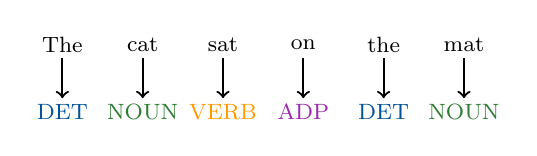
\begin{tikzpicture}[scale=0.85]
            \node[font=\footnotesize] at (0,1) {The};
            \node[font=\footnotesize] at (1.2,1) {cat};
            \node[font=\footnotesize] at (2.4,1) {sat};
            \node[font=\footnotesize] at (3.6,1) {on};
            \node[font=\footnotesize] at (4.8,1) {the};
            \node[font=\footnotesize] at (6,1) {mat};

            \draw[->, thick] (0,0.8) -- (0,0.2);
            \draw[->, thick] (1.2,0.8) -- (1.2,0.2);
            \draw[->, thick] (2.4,0.8) -- (2.4,0.2);
            \draw[->, thick] (3.6,0.8) -- (3.6,0.2);
            \draw[->, thick] (4.8,0.8) -- (4.8,0.2);
            \draw[->, thick] (6,0.8) -- (6,0.2);

            \node[font=\footnotesize, color=darkblue] at (0,0) {DET};
            \node[font=\footnotesize, color=darkgreen] at (1.2,0) {NOUN};
            \node[font=\footnotesize, color=orange] at (2.4,0) {VERB};
            \node[font=\footnotesize, color=purple] at (3.6,0) {ADP};
            \node[font=\footnotesize, color=darkblue] at (4.8,0) {DET};
            \node[font=\footnotesize, color=darkgreen] at (6,0) {NOUN};
        \end{tikzpicture}
    \end{center}

    \vspace{0.5em}
    \textbf{Why it matters:}
    \begin{itemize}\setlength{\itemsep}{0pt}
        \item Disambiguation: "book" as noun vs. verb
        \item Syntax parsing and understanding
        \item Information extraction, machine translation
    \end{itemize}
\end{frame}

\begin{frame}[shrink=10]{POS Tagsets: Universal vs. Fine-Grained 📋}
    \begin{columns}[T]
        \begin{column}{0.48\textwidth}
            \textbf{Universal POS Tags (17 tags):}
            \begin{itemize}\setlength{\itemsep}{0pt}
                \item ADJ: adjective
                \item ADP: adposition
                \item ADV: adverb
                \item AUX: auxiliary
                \item CONJ: conjunction
                \item DET: determiner
                \item NOUN: noun
                \item NUM: numeral
                \item PRON: pronoun
                \item PROPN: proper noun
                \item VERB: verb
                \item ...
            \end{itemize}
        \end{column}
        \begin{column}{0.48\textwidth}
            \textbf{Penn Treebank (45+ tags):}
            \begin{itemize}\setlength{\itemsep}{0pt}
                \item NN: noun, singular
                \item NNS: noun, plural
                \item NNP: proper noun, singular
                \item NNPS: proper noun, plural
                \item VB: verb, base form
                \item VBD: verb, past tense
                \item VBG: verb, gerund
                \item VBN: verb, past participle
                \item VBP: verb, non-3rd person
                \item VBZ: verb, 3rd person
                \item ...
            \end{itemize}
        \end{column}
    \end{columns}

    \vspace{0.5em}
    \textbf{Trade-off:} Simplicity vs. linguistic detail
\end{frame}

\begin{frame}{Context Matters: Ambiguous Words 🔄}
    \textbf{Many words have multiple possible POS tags:}

    \vspace{0.5em}
    \begin{center}
        \begin{tabular}{lll}
            \toprule
            \textbf{Sentence} & \textbf{Word} & \textbf{POS} \\
            \midrule
            "I \textbf{book} a flight" & book & VERB \\
            "I read a \textbf{book}" & book & NOUN \\
            \midrule
            "The \textbf{fast} car" & fast & ADJ \\
            "She runs \textbf{fast}" & fast & ADV \\
            "I will \textbf{fast} today" & fast & VERB \\
            \midrule
            "The meeting is \textbf{close}" & close & ADJ \\
            "Please \textbf{close} the door" & close & VERB \\
            \bottomrule
        \end{tabular}
    \end{center}

    \vspace{0.5em}
    \textbf{Key insight:} Context determines POS! Models must look at surrounding words.
\end{frame}

\begin{frame}[fragile]{POS Tagging with spaCy 🚀}
    \begin{lstlisting}[language=Python]
import spacy

nlp = spacy.load("en_core_web_sm")

sentence = "She will book the meeting room tomorrow"
doc = nlp(sentence)

print(f"{'Word':<12} {'POS':<8} {'Detailed Tag':<12} {'Explanation'}")
print("-" * 55)
for token in doc:
    explanation = spacy.explain(token.pos_)
    print(f"{token.text:<12} {token.pos_:<8} {token.tag_:<12} {explanation}")

# Output:
# Word         POS      Detailed Tag  Explanation
# -------------------------------------------------------
# She          PRON     PRP           pronoun, personal
# will         AUX      MD            verb, modal auxiliary
# book         VERB     VB            verb, base form
# the          DET      DT            determiner
# meeting      NOUN     NN            noun, singular or mass
# room         NOUN     NN            noun, singular or mass
# tomorrow     NOUN     NN            noun, singular or mass
    \end{lstlisting}

    Notice: "book" correctly identified as VERB! ✅
\end{frame}

\begin{frame}[shrink=10]{How Do POS Taggers Work? 🧠}
    \textbf{Traditional approaches (pre-neural):}
    \begin{itemize}\setlength{\itemsep}{0pt}
        \item Rule-based: Hand-crafted grammar rules
        \item Hidden Markov Models (HMMs): Probabilistic sequences
        \item Conditional Random Fields (CRFs): Structured prediction
    \end{itemize}

    \vspace{0.5em}
    \textbf{Modern neural approaches:}
    \begin{itemize}\setlength{\itemsep}{0pt}
        \item Recurrent Neural Networks (RNNs/LSTMs): Process sequences
        \item Transformers (BERT, etc.): Bidirectional context
        \item Fine-tune pre-trained models on POS data
    \end{itemize}

    \vspace{0.5em}
    \textbf{Advantages of neural methods:}
    \begin{itemize}\setlength{\itemsep}{0pt}
        \item Learn patterns from data (no hand-crafted rules)
        \item Capture long-range dependencies
        \item Handle ambiguity through context
        \item State-of-the-art accuracy (>97% on English!)
    \end{itemize}
\end{frame}

\begin{frame}{Neural Networks and Grammar 🤖}
    \textbf{Can neural networks learn syntactic structure?}

    \vspace{0.5em}
    \textbf{Classic test:} Subject-verb agreement (Linzen et al., 2016)

    \begin{center}
        \begin{tikzpicture}[scale=0.85]
            \node[align=left, font=\footnotesize] at (0,2) {
                "The key to the cabinets \textcolor{darkgreen}{\textbf{is}} on the table" ✅
            };
            \node[align=left, font=\footnotesize] at (0,1) {
                "The key to the cabinets \textcolor{lightred}{\textbf{are}} on the table" ❌
            };

            \draw[decorate, decoration={brace, amplitude=5pt}, thick] (-3.5,0.5) -- (-3.5,2.5);
            \node[left, font=\tiny, align=right] at (-3.7,1.5) {Must track\\"key" not\\"cabinets"};
        \end{tikzpicture}
    \end{center}

    \vspace{0.5em}
    \textbf{Challenge:} Distractor nouns between subject and verb

    \begin{itemize}\setlength{\itemsep}{0pt}
        \item Model must identify "key" (singular) as subject
        \item Ignore "cabinets" (plural distractor)
        \item Predict correct verb form "is" (not "are")
    \end{itemize}

    \vspace{0.5em}
    \textbf{Finding:} LSTMs can learn this! But they struggle with complex cases.

    \vspace{0.3em}
    📖 \textbf{Reference:} Linzen, Dupoux, \& Goldberg (2016). Assessing the Ability of LSTMs to Learn Syntax-Sensitive Dependencies. \textit{TACL}.
\end{frame}

\begin{frame}{BLiMP: Testing Linguistic Knowledge 📊}
    \textbf{BLiMP Dataset} (Warstadt et al., 2020):
    \begin{itemize}\setlength{\itemsep}{0pt}
        \item Benchmark of Linguistic Minimal Pairs
        \item 67,000 sentence pairs across 67 paradigms
        \item Tests syntax, semantics, morphology
    \end{itemize}

    \vspace{0.5em}
    \textbf{Example minimal pairs:}

    \begin{center}
        \begin{tabular}{ll}
            \toprule
            \textbf{Acceptable} & \textbf{Unacceptable} \\
            \midrule
            "The author writes" & "The author write" \\
            "Who did you see?" & "Who did you saw?" \\
            "I think that she left" & "I think that she leave" \\
            \bottomrule
        \end{tabular}
    \end{center}

    \vspace{0.5em}
    \textbf{Task:} Model should assign higher probability to acceptable sentence

    \vspace{0.5em}
    \textbf{Results:} Transformers (BERT, GPT-2) perform well (70-85%), but not perfect!

    \vspace{0.3em}
    📖 \textbf{Reference:} Warstadt et al. (2020). BLiMP: The Benchmark of Linguistic Minimal Pairs. \textit{TACL}.
\end{frame}

\begin{frame}[fragile]{Token Classification with HuggingFace 🤗}
    \begin{lstlisting}[language=Python]
from transformers import pipeline

# Load POS tagging pipeline (or NER, etc.)
pos_tagger = pipeline("token-classification",
                      model="vblagoje/bert-english-uncased-finetuned-pos",
                      aggregation_strategy="simple")

sentence = "Apple Inc. is looking at buying a UK startup"
results = pos_tagger(sentence)

for result in results:
    print(f"{result['word']:<15} {result['entity_group']:<8} "
          f"(confidence: {result['score']:.3f})")

# Output:
# Apple           PROPN    (confidence: 0.998)
# Inc.            PROPN    (confidence: 0.995)
# is              AUX      (confidence: 0.999)
# looking         VERB     (confidence: 0.997)
# at              ADP      (confidence: 0.999)
# ...
    \end{lstlisting}

    📖 \href{https://huggingface.co/learn/nlp-course/chapter7/2}{HuggingFace Chapter 7.2: Token Classification}
\end{frame}

\begin{frame}[shrink=10]{Discussion: Do Models "Understand" Grammar? 🤔}
    \textbf{Perspectives to consider:}

    \begin{enumerate}\setlength{\itemsep}{0pt}
        \item \textbf{Chomsky's view:} Grammar requires innate, symbolic rules
        \begin{itemize}\setlength{\itemsep}{0pt}
            \item Can statistical patterns truly capture grammatical knowledge?
        \end{itemize}

        \item \textbf{Emergentist view:} Grammar emerges from usage patterns
        \begin{itemize}\setlength{\itemsep}{0pt}
            \item Maybe neural networks learn similarly to humans?
        \end{itemize}

        \item \textbf{Functional perspective:} If it works, does it matter?
        \begin{itemize}\setlength{\itemsep}{0pt}
            \item Models perform well on tasks—is that "understanding"?
        \end{itemize}

        \item \textbf{Limitations:} Models still fail on edge cases
        \begin{itemize}\setlength{\itemsep}{0pt}
            \item What does this tell us about their knowledge?
        \end{itemize}
    \end{enumerate}

    \vspace{0.5em}
    \textbf{Your thoughts?} Is pattern matching sufficient for grammatical competence?
\end{frame}

% Part 2: Sentiment Analysis
\begin{frame}[shrink=10]{Sentiment Analysis: From Structure to Emotion 😊😢}
    \textbf{What is sentiment analysis?}
    \begin{itemize}\setlength{\itemsep}{0pt}
        \item Determining emotional tone of text
        \item Classification task: positive, negative, neutral (or fine-grained)
        \item Moves beyond structure to \textit{meaning}
    \end{itemize}

    \vspace{0.5em}
    \textbf{Applications:}
    \begin{itemize}\setlength{\itemsep}{0pt}
        \item 📱 Social media monitoring
        \item 🛍️ Customer feedback analysis
        \item 📈 Market research and stock prediction
        \item 🎬 Movie/product review analysis
        \item 🗳️ Political opinion tracking
    \end{itemize}

    \vspace{0.5em}
    \textbf{Granularity levels:}
    \begin{itemize}\setlength{\itemsep}{0pt}
        \item Binary: positive vs. negative
        \item Ternary: positive, negative, neutral
        \item Fine-grained: 1-5 stars, or continuous score
    \end{itemize}
\end{frame}

\begin{frame}[shrink=10]{Sentiment Analysis Challenges 🚧}
    \textbf{1. Sarcasm and irony:}
    \begin{itemize}\setlength{\itemsep}{0pt}
        \item "Oh great, another meeting 🙄" (negative, despite "great")
        \item "This is the best movie I've ever fallen asleep to" (negative!)
    \end{itemize}

    \vspace{0.3em}
    \textbf{2. Context-dependent sentiment:}
    \begin{itemize}\setlength{\itemsep}{0pt}
        \item "This movie is sick!" (positive in slang, negative literally)
        \item "The book was long" (neutral? negative?)
    \end{itemize}

    \vspace{0.3em}
    \textbf{3. Mixed sentiment:}
    \begin{itemize}\setlength{\itemsep}{0pt}
        \item "Great food but terrible service" (both positive and negative)
        \item Aspect-based sentiment: food=positive, service=negative
    \end{itemize}

    \vspace{0.3em}
    \textbf{4. Negation:}
    \begin{itemize}\setlength{\itemsep}{0pt}
        \item "not good" vs. "good"
        \item "I don't dislike it" (double negative = positive?)
    \end{itemize}

    \vspace{0.3em}
    \textbf{5. Domain specificity:}
    \begin{itemize}\setlength{\itemsep}{0pt}
        \item "Explosive growth" (positive in business, negative in safety)
        \item Different domains have different sentiment patterns
    \end{itemize}
\end{frame}

\begin{frame}{Sentiment Lexicons: The Old-School Approach 📖}
    \textbf{Traditional method:} Dictionary of words with sentiment scores

    \vspace{0.5em}
    \textbf{Popular lexicons:}
    \begin{itemize}\setlength{\itemsep}{0pt}
        \item \textbf{AFINN:} Words rated from -5 (very negative) to +5 (very positive)
        \item \textbf{SentiWordNet:} Assigns positive/negative/neutral scores
        \item \textbf{VADER:} Designed for social media text (handles emoji, slang)
    \end{itemize}

    \vspace{0.5em}
    \textbf{Example (AFINN):}
    \begin{center}
        \begin{tabular}{ll}
            \toprule
            \textbf{Word} & \textbf{Score} \\
            \midrule
            love & +3 \\
            great & +3 \\
            good & +3 \\
            hate & -3 \\
            terrible & -3 \\
            awful & -3 \\
            \bottomrule
        \end{tabular}
    \end{center}

    \vspace{0.3em}
    \textbf{Limitations:} Ignores context, word order, sarcasm...
\end{frame}

\begin{frame}[fragile]{Lexicon-Based Sentiment Analysis 🔤}
    \begin{lstlisting}[language=Python]
from vaderSentiment.vaderSentiment import SentimentIntensityAnalyzer

analyzer = SentimentIntensityAnalyzer()

texts = [
    "I love this product! It's amazing!",
    "This is the worst experience ever.",
    "It's okay, nothing special.",
    "Great food but terrible service! 😊😢"
]

for text in texts:
    scores = analyzer.polarity_scores(text)
    print(f"Text: {text}")
    print(f"  Positive: {scores['pos']:.2f}, "
          f"Negative: {scores['neg']:.2f}, "
          f"Neutral: {scores['neu']:.2f}")
    print(f"  Compound: {scores['compound']:.3f}\n")

# VADER handles emoji and punctuation!
# "Great!!!" has higher positive score than "Great"
    \end{lstlisting}
\end{frame}

\begin{frame}[fragile]{Modern Approach: Pre-trained Models 🤖}
    \textbf{Neural network advantages:}
    \begin{itemize}\setlength{\itemsep}{0pt}
        \item Learn context-dependent representations
        \item Capture word order and negation
        \item Handle sarcasm better (though still imperfect)
        \item Transfer learning: pre-train on large corpus, fine-tune for sentiment
    \end{itemize}

    \vspace{0.5em}
    \textbf{Typical architecture:}
    \begin{center}
        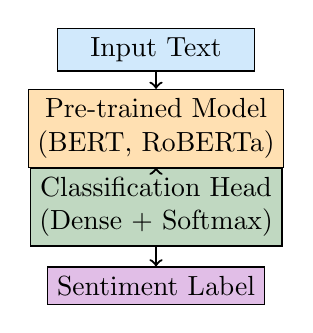
\begin{tikzpicture}[scale=0.85][node distance=1.5cm]
            \node[rectangle, draw, fill=lightblue!30, minimum width=2.5cm] (input) {Input Text};
            \node[rectangle, draw, fill=orange!30, minimum width=2.5cm, below of=input, align=center] (bert) {Pre-trained Model\\(BERT, RoBERTa)};
            \node[rectangle, draw, fill=darkgreen!30, minimum width=2.5cm, below of=bert, align=center] (cls) {Classification Head\\(Dense + Softmax)};
            \node[rectangle, draw, fill=purple!30, minimum width=2.5cm, below of=cls] (output) {Sentiment Label};

            \draw[->, thick] (input) -- (bert);
            \draw[->, thick] (bert) -- (cls);
            \draw[->, thick] (cls) -- (output);
        \end{tikzpicture}
    \end{center}

    \vspace{0.5em}
    \textbf{Training:} Fine-tune on labeled sentiment data (IMDb, Amazon reviews, etc.)
\end{frame}

\begin{frame}[fragile]{Sentiment Analysis with HuggingFace 🤗}
    \begin{lstlisting}[language=Python]
from transformers import pipeline

# Load pre-trained sentiment analysis pipeline
sentiment_analyzer = pipeline("sentiment-analysis")

texts = [
    "I love this product! It's amazing!",
    "This is the worst experience ever.",
    "It's okay, nothing special.",
    "I don't hate it, but I don't love it either."
]

for text in texts:
    result = sentiment_analyzer(text)[0]
    print(f"Text: {text}")
    print(f"  Sentiment: {result['label']}, "
          f"Confidence: {result['score']:.3f}\n")

# Output:
# Text: I love this product! It's amazing!
#   Sentiment: POSITIVE, Confidence: 0.999
#
# Text: This is the worst experience ever.
#   Sentiment: NEGATIVE, Confidence: 0.998
    \end{lstlisting}

    📖 \href{https://huggingface.co/learn/nlp-course/chapter1/2}{HuggingFace Chapter 1.2: NLP Tasks}
\end{frame}

\begin{frame}{Domain-Specific Sentiment Models 🎯}
    \textbf{Problem:} General models may not understand domain-specific language

    \vspace{0.5em}
    \textbf{Solution:} Fine-tune on domain-specific data!

    \vspace{0.5em}
    \begin{table}
        \centering
        \small
        \begin{tabular}{lll}
            \toprule
            \textbf{Domain} & \textbf{Model} & \textbf{Example Use} \\
            \midrule
            Financial & FinBERT & Earnings sentiment \\
            Medical & BioBERT + fine-tune & Patient feedback \\
            Twitter & TwitterBERT & Social monitoring \\
            Product Reviews & RoBERTa + Amazon & E-commerce \\
            Movies & BERT + IMDb & Film reviews \\
            \bottomrule
        \end{tabular}
    \end{table}

    \vspace{0.5em}
    \textbf{Why it works:}
    \begin{itemize}\setlength{\itemsep}{0pt}
        \item Domain-specific vocabulary ("bullish" in finance = positive)
        \item Different sentiment expressions
        \item Adapted to domain conventions
    \end{itemize}
\end{frame}

\begin{frame}[fragile]{Comparing General vs. Domain-Specific 📊}
    \begin{lstlisting}[language=Python]
from transformers import pipeline

# General sentiment model
general = pipeline("sentiment-analysis")

# Financial sentiment model
financial = pipeline("sentiment-analysis",
                    model="ProsusAI/finbert")

texts = [
    "The company's earnings exceeded expectations",
    "Revenue declined but margins improved",
    "Stock prices plummeted amid uncertainty"
]

for text in texts:
    gen_result = general(text)[0]
    fin_result = financial(text)[0]

    print(f"Text: {text}")
    print(f"  General: {gen_result['label']} ({gen_result['score']:.3f})")
    print(f"  Financial: {fin_result['label']} ({fin_result['score']:.3f})\n")

# Financial model often more accurate for finance text!
    \end{lstlisting}
\end{frame}

\begin{frame}[shrink=10]{Fine-Tuning for Sentiment Analysis 🎓}
    \textbf{Process overview:}

    \begin{enumerate}\setlength{\itemsep}{0pt}
        \item \textbf{Start with pre-trained model} (e.g., BERT, RoBERTa)
        \begin{itemize}\setlength{\itemsep}{0pt}
            \item Already knows language structure from pre-training
        \end{itemize}

        \item \textbf{Prepare labeled dataset}
        \begin{itemize}\setlength{\itemsep}{0pt}
            \item Text + sentiment labels (positive/negative/neutral)
            \item Examples: IMDb reviews, Amazon products, Twitter data
        \end{itemize}

        \item \textbf{Add classification head}
        \begin{itemize}\setlength{\itemsep}{0pt}
            \item Dense layer on top of model
            \item Outputs: probability distribution over classes
        \end{itemize}

        \item \textbf{Fine-tune on sentiment data}
        \begin{itemize}\setlength{\itemsep}{0pt}
            \item Update model weights to predict sentiment
            \item Much faster than training from scratch!
        \end{itemize}

        \item \textbf{Evaluate on test set}
        \begin{itemize}\setlength{\itemsep}{0pt}
            \item Accuracy, precision, recall, F1-score
        \end{itemize}
    \end{enumerate}

    📖 \href{https://huggingface.co/learn/nlp-course/chapter3/2}{HuggingFace Chapter 3.2: Processing Data for Fine-tuning}
\end{frame}

\begin{frame}[fragile]{Fine-Tuning Example (Simplified) 🔧}
    \begin{lstlisting}[language=Python]
from transformers import AutoModelForSequenceClassification, Trainer

# 1. Load pre-trained model
model = AutoModelForSequenceClassification.from_pretrained(
    "bert-base-uncased",
    num_labels=2  # positive/negative
)

# 2. Prepare data (tokenized with labels)
# train_dataset, eval_dataset = ... (omitted for brevity)

# 3. Define training arguments
training_args = TrainingArguments(
    output_dir="./results",
    num_train_epochs=3,
    per_device_train_batch_size=16,
    evaluation_strategy="epoch"
)

# 4. Create Trainer and train
trainer = Trainer(
    model=model,
    args=training_args,
    train_dataset=train_dataset,
    eval_dataset=eval_dataset
)

trainer.train()
    \end{lstlisting}
\end{frame}

\begin{frame}[shrink=10]{Evaluation Metrics for Sentiment Analysis 📏}
    \textbf{Beyond accuracy:}

    \begin{itemize}\setlength{\itemsep}{0pt}
        \item \textbf{Precision:} Of predicted positives, how many are truly positive?
        \[
        \text{Precision} = \frac{\text{True Positives}}{\text{True Positives} + \text{False Positives}}
        \]

        \item \textbf{Recall:} Of actual positives, how many did we catch?
        \[
        \text{Recall} = \frac{\text{True Positives}}{\text{True Positives} + \text{False Negatives}}
        \]

        \item \textbf{F1-Score:} Harmonic mean of precision and recall
        \[
        F1 = 2 \times \frac{\text{Precision} \times \text{Recall}}{\text{Precision} + \text{Recall}}
        \]
    \end{itemize}

    \vspace{0.5em}
    \textbf{Why not just accuracy?}
    \begin{itemize}\setlength{\itemsep}{0pt}
        \item Imbalanced datasets (e.g., 90\% positive reviews)
        \item Different costs for false positives vs. false negatives
        \item F1 gives balanced view of model performance
    \end{itemize}
\end{frame}

\begin{frame}[shrink=5]{Confusion Matrix Example 🎭}
    \begin{center}
        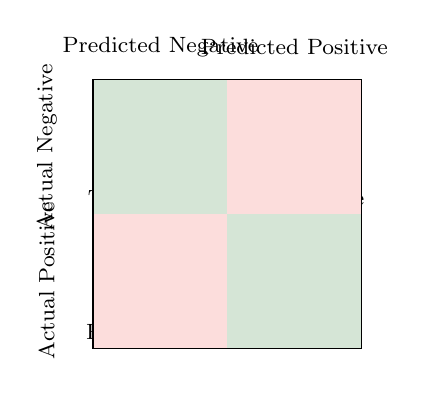
\begin{tikzpicture}[scale=0.85]
            % Matrix
            \draw[thick] (0,0) rectangle (4,4);
            \draw[thick] (0,2) -- (4,2);
            \draw[thick] (2,0) -- (2,4);

            % Labels
            \node[font=\footnotesize] at (1,4.5) {Predicted Negative};
            \node[font=\footnotesize] at (3,4.5) {Predicted Positive};
            \node[font=\footnotesize, rotate=90] at (-0.7,3) {Actual Negative};
            \node[font=\footnotesize, rotate=90] at (-0.7,1) {Actual Positive};

            % Values
            \node[font=\Large] at (1,3) {850};
            \node[font=\footnotesize, below] at (1,2.5) {True Negative};

            \node[font=\Large] at (3,3) {50};
            \node[font=\footnotesize, below] at (3,2.5) {False Positive};

            \node[font=\Large] at (1,1) {100};
            \node[font=\footnotesize, below] at (1,0.5) {False Negative};

            \node[font=\Large] at (3,1) {900};
            \node[font=\footnotesize, below] at (3,0.5) {True Positive};

            % Color coding
            \fill[darkgreen!20] (2,0) rectangle (4,2);
            \fill[darkgreen!20] (0,2) rectangle (2,4);
            \fill[lightred!20] (0,0) rectangle (2,2);
            \fill[lightred!20] (2,2) rectangle (4,4);
        \end{tikzpicture}
    \end{center}

    \vspace{0.3em}
    Accuracy = 92\% | Precision = 95\% | Recall = 90\% | F1 = 92\%
\end{frame}

\begin{frame}[shrink=10]{Aspect-Based Sentiment Analysis 🔍}
    \textbf{Problem:} Reviews often mention multiple aspects with different sentiments

    \vspace{0.5em}
    \textbf{Example:}
    \begin{quote}
        "The \textcolor{darkgreen}{food was delicious} but the \textcolor{lightred}{service was terrible}. The \textcolor{orange}{atmosphere was okay}."
    \end{quote}

    \vspace{0.5em}
    \textbf{Aspect-based approach:}
    \begin{itemize}\setlength{\itemsep}{0pt}
        \item Food: \textcolor{darkgreen}{Positive} ✅
        \item Service: \textcolor{lightred}{Negative} ❌
        \item Atmosphere: \textcolor{orange}{Neutral} 😐
    \end{itemize}

    \vspace{0.5em}
    \textbf{Applications:}
    \begin{itemize}\setlength{\itemsep}{0pt}
        \item Restaurant reviews: food, service, ambiance, price
        \item Product reviews: quality, price, shipping, customer service
        \item Hotel reviews: room, location, staff, cleanliness
    \end{itemize}

    \vspace{0.5em}
    \textbf{More nuanced than overall sentiment!} Provides actionable insights.
\end{frame}

\begin{frame}[shrink=5]{Real-World Application: Product Review Analysis 🛍️}
    \textbf{Business value:}
    \begin{itemize}\setlength{\itemsep}{0pt}
        \item Identify product strengths and weaknesses
        \item Track sentiment trends over time
        \item Compare against competitors
        \item Prioritize product improvements
    \end{itemize}

    \vspace{0.5em}
    \textbf{Example insights from Amazon reviews:}
    \begin{center}
        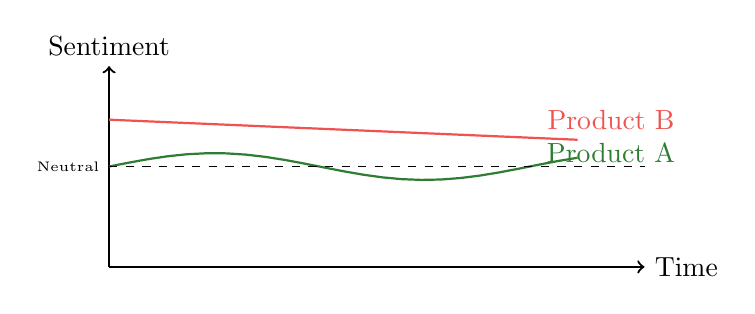
\begin{tikzpicture}[scale=0.85]
            \draw[->, thick] (0,0) -- (8,0) node[right] {Time};
            \draw[->, thick] (0,0) -- (0,3) node[above] {Sentiment};

            % Product 1
            \draw[thick, color=darkgreen, domain=0:7] plot (\x, {1.5 + 0.2*sin(\x r)});
            \node[color=darkgreen] at (7.5,1.7) {Product A};

            % Product 2
            \draw[thick, color=lightred, domain=0:7] plot (\x, {2.2 - 0.3*\x/7});
            \node[color=lightred] at (7.5,2.2) {Product B};

            \draw[dashed] (0,1.5) -- (8,1.5);
            \node[left, font=\tiny] at (0,1.5) {Neutral};
        \end{tikzpicture}
    \end{center}

    Product A: Stable positive sentiment

    Product B: Declining sentiment → investigate quality issues!
\end{frame}

\begin{frame}[shrink=10]{Hands-On Exercise 🧪}
    \textbf{Try this yourself:}

    \begin{enumerate}\setlength{\itemsep}{0pt}
        \item \textbf{Collect data:}
        \begin{itemize}\setlength{\itemsep}{0pt}
            \item Scrape product reviews (Amazon, Yelp)
            \item Or use public dataset (IMDb, Twitter)
        \end{itemize}

        \item \textbf{Compare approaches:}
        \begin{itemize}\setlength{\itemsep}{0pt}
            \item Lexicon-based (VADER)
            \item General pre-trained model (HuggingFace pipeline)
            \item Domain-specific model (if available)
        \end{itemize}

        \item \textbf{Analyze results:}
        \begin{itemize}\setlength{\itemsep}{0pt}
            \item Where do models disagree?
            \item Which handles sarcasm better?
            \item Which is most accurate for your domain?
        \end{itemize}

        \item \textbf{Bonus:} Fine-tune a model on your specific dataset!
    \end{enumerate}
\end{frame}

\begin{frame}[shrink=10]{Discussion: Understanding Emotion 💭}
    \textbf{Philosophical questions:}

    \begin{enumerate}\setlength{\itemsep}{0pt}
        \item \textbf{Can models "feel" sentiment?}
        \begin{itemize}\setlength{\itemsep}{0pt}
            \item They predict labels, but do they understand emotion?
        \end{itemize}

        \item \textbf{Is sentiment objective or subjective?}
        \begin{itemize}\setlength{\itemsep}{0pt}
            \item Different annotators may disagree on sentiment
            \item How do models handle ambiguity?
        \end{itemize}

        \item \textbf{Cultural and linguistic variation:}
        \begin{itemize}\setlength{\itemsep}{0pt}
            \item Sentiment expressions vary across cultures
            \item Can models capture these nuances?
        \end{itemize}

        \item \textbf{Ethical considerations:}
        \begin{itemize}\setlength{\itemsep}{0pt}
            \item Automated sentiment analysis in hiring, lending...
            \item Risks of bias and discrimination
            \item Should we trust model judgments?
        \end{itemize}
    \end{enumerate}
\end{frame}

% Week 2 Wrap-up
\begin{frame}[shrink=5]{Week 2 Integration: Putting It All Together 🧩}
    \textbf{How the pieces connect:}

    \begin{center}
        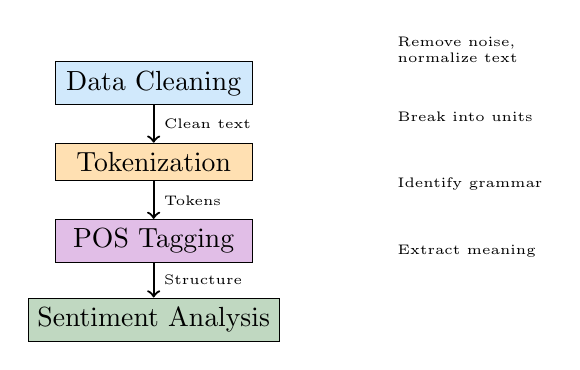
\begin{tikzpicture}[scale=0.85][node distance=1cm]
            \node[rectangle, draw, fill=lightblue!30, minimum width=2.5cm] (clean) {Data Cleaning};
            \node[rectangle, draw, fill=orange!30, minimum width=2.5cm, below of=clean] (token) {Tokenization};
            \node[rectangle, draw, fill=purple!30, minimum width=2.5cm, below of=token] (pos) {POS Tagging};
            \node[rectangle, draw, fill=darkgreen!30, minimum width=2.5cm, below of=pos] (sent) {Sentiment Analysis};

            \draw[->, thick] (clean) -- (token) node[midway,right,font=\tiny] {Clean text};
            \draw[->, thick] (token) -- (pos) node[midway,right,font=\tiny] {Tokens};
            \draw[->, thick] (pos) -- (sent) node[midway,right,font=\tiny] {Structure};

            \node[right, font=\tiny, align=left] at (3.5,0.5) {Remove noise,\\normalize text};
            \node[right, font=\tiny, align=left] at (3.5,-0.5) {Break into units};
            \node[right, font=\tiny, align=left] at (3.5,-1.5) {Identify grammar};
            \node[right, font=\tiny, align=left] at (3.5,-2.5) {Extract meaning};
        \end{tikzpicture}
    \end{center}

    \vspace{0.5em}
    Each step builds on the previous one!
\end{frame}

\begin{frame}[shrink=10]{Assignment 2: SPAM Email Classifier 📧}
    \textbf{Your task:} Build a classifier to detect spam emails

    \vspace{0.5em}
    \textbf{Apply this week's concepts:}
    \begin{itemize}\setlength{\itemsep}{0pt}
        \item \textbf{Data cleaning:} Remove HTML tags, normalize text
        \item \textbf{Tokenization:} Try different tokenizers (word, subword)
        \item \textbf{Features:} Extract useful signals (POS patterns, sentiment?)
        \item \textbf{Classification:} Train a model to identify spam
    \end{itemize}

    \vspace{0.5em}
    \textbf{Think about:}
    \begin{itemize}\setlength{\itemsep}{0pt}
        \item What makes spam different from legitimate emails?
        \item How does preprocessing affect accuracy?
        \item Can you use sentiment as a feature?
        \item What about POS patterns? (e.g., spam has more imperatives?)
    \end{itemize}

    \vspace{0.5em}
    \textbf{Link:} \href{https://github.com/ContextLab/llm-course/tree/main/assignments/Assignment\%202\%3A\%20SPAM\%20classifier}{Assignment 2: SPAM classifier}
\end{frame}

\begin{frame}[shrink=10]{Key Takeaways 🎯}
    \begin{enumerate}\setlength{\itemsep}{0pt}
        \item \textbf{POS tagging reveals grammatical structure}
        \begin{itemize}\setlength{\itemsep}{0pt}
            \item Neural networks can learn syntax from data
            \item But do they "understand" grammar? Debatable!
        \end{itemize}

        \item \textbf{Sentiment analysis extracts emotional meaning}
        \begin{itemize}\setlength{\itemsep}{0pt}
            \item From lexicons to neural networks
            \item Domain-specific fine-tuning improves accuracy
        \end{itemize}

        \item \textbf{Statistical learning powers modern NLP}
        \begin{itemize}\setlength{\itemsep}{0pt}
            \item Models learn patterns without explicit rules
            \item Similar to how infants learn language?
        \end{itemize}

        \item \textbf{Context is crucial}
        \begin{itemize}\setlength{\itemsep}{0pt}
            \item Words are ambiguous—meaning comes from context
            \item Transformers excel at capturing context
        \end{itemize}

        \item \textbf{Critical thinking matters}
        \begin{itemize}\setlength{\itemsep}{0pt}
            \item Question what "understanding" means
            \item Be aware of limitations and biases
        \end{itemize}
    \end{enumerate}
\end{frame}

\begin{frame}[shrink=10]{Primary References 📚}
    \textbf{POS Tagging and Syntax:}
    \begin{itemize}\setlength{\itemsep}{0pt}
        \item Linzen, Dupoux, \& Goldberg (2016). Assessing the Ability of LSTMs to Learn Syntax-Sensitive Dependencies. \textit{TACL}.
        \item Warstadt et al. (2020). BLiMP: The Benchmark of Linguistic Minimal Pairs. \textit{TACL}.
    \end{itemize}

    \vspace{0.3em}
    \textbf{Sentiment Analysis:}
    \begin{itemize}\setlength{\itemsep}{0pt}
        \item Pang \& Lee (2008). Opinion Mining and Sentiment Analysis. \textit{Foundations and Trends in IR}.
        \item Hutto \& Gilbert (2014). VADER: A Parsimonious Rule-based Model for Sentiment Analysis. \textit{ICWSM}.
    \end{itemize}

    \vspace{0.3em}
    \textbf{HuggingFace Resources:}
    \begin{itemize}\setlength{\itemsep}{0pt}
        \item \href{https://huggingface.co/learn/nlp-course/chapter1/2}{Chapter 1.2: NLP Tasks with Pipeline}
        \item \href{https://huggingface.co/learn/nlp-course/chapter3/2}{Chapter 3.2: Processing Data for Fine-tuning}
        \item \href{https://huggingface.co/learn/nlp-course/chapter7/2}{Chapter 7.2: Token Classification}
    \end{itemize}
\end{frame}

\begin{frame}[shrink=10]{Looking Ahead: Weeks 3-4 🔮}
    \textbf{Next topics:}
    \begin{itemize}\setlength{\itemsep}{0pt}
        \item Dimensionality reduction (PCA, UMAP)
        \item Bag-of-words and TF-IDF
        \item Word embeddings (Word2Vec, GloVe)
        \item Distributional semantics
    \end{itemize}

    \vspace{1em}
    \textbf{Central question:}
    \begin{center}
        \textit{"You shall know a word by the company it keeps"}
    \end{center}

    How can we represent word \textit{meaning} computationally?

    \vspace{1em}
    \textbf{Prepare by:}
    \begin{itemize}\setlength{\itemsep}{0pt}
        \item Completing Assignment 2
        \item Thinking about: What is "meaning"? How would you define it?
        \item Exploring: Vector representations and semantic similarity
    \end{itemize}
\end{frame}

\begin{frame}[shrink=10]{Additional Resources 🔗}
    \textbf{Tools and libraries:}
    \begin{itemize}\setlength{\itemsep}{0pt}
        \item spaCy: \url{https://spacy.io/}
        \item HuggingFace Transformers: \url{https://huggingface.co/docs/transformers/}
        \item VADER Sentiment: \url{https://github.com/cjhutto/vaderSentiment}
    \end{itemize}

    \vspace{0.5em}
    \textbf{Datasets:}
    \begin{itemize}\setlength{\itemsep}{0pt}
        \item IMDb Movie Reviews: \url{https://ai.stanford.edu/~amaas/data/sentiment/}
        \item Amazon Product Reviews: \url{https://registry.opendata.aws/amazon-reviews/}
        \item Stanford Sentiment Treebank: \url{https://nlp.stanford.edu/sentiment/}
    \end{itemize}

    \vspace{0.5em}
    \textbf{Interactive demos:}
    \begin{itemize}\setlength{\itemsep}{0pt}
        \item HuggingFace Spaces: Try models in your browser!
        \item \url{https://huggingface.co/spaces}
    \end{itemize}
\end{frame}

\begin{frame}[standout]
    \Huge Thank you! 🎉

    \vspace{1em}

    \large Questions?

    \vspace{1em}

    \normalsize
    Week 2 complete! See you in Week 3!

    \vspace{0.5em}

    Happy coding! 💻
\end{frame}

\end{document}
